\documentclass[handout,xcolor={dvipsnames}]{beamer}
% MD: we can mess with this ...
%\usetheme{Berlin}
%\usetheme{Goettingen}
% ... or use the IU style we've defined before:
%\usepackage{iucl}
%\usepackage[dvipsnames]{xcolor}
\usepackage{array}
\usepackage{graphicx}
\usepackage{tikz-dependency}
\usepackage{natbib}
\usepackage{url}
\usepackage{gb4e}
\usepackage{tikz-qtree}
%\usepackage{caption}

\makeatletter

\newcommand*{\@rowstyle}{}

\newcommand*{\rowstyle}[1]{% sets the style of the next row
  \gdef\@rowstyle{#1}%
  \@rowstyle\ignorespaces%
}

\newcolumntype{=}{% resets the row style
  >{\gdef\@rowstyle{}}%
}

\newcolumntype{+}{% adds the current row style to the next column
  >{\@rowstyle}%
}

\makeatother

%%%
\setbeamertemplate{itemize/enumerate body begin}{\small}
\setbeamertemplate{itemize/enumerate subbody begin}{\small}
\setbeamertemplate{itemize/enumerate subsubbody begin}{\small}
%%%



% workaround for weird \newblock problem
% http://www.isi.edu/~johnh/SOFTWARE/uclathes.html
\def\newblock{\hskip .11em plus .33em minus .07em}

% MD: changing tables so we don't need these
\usepackage{multirow}
% \usepackage{rotating}
% \usepackage{booktabs}

\title{Semantic Analysis of Image-Based Learner Sentences}
\author[Levi King]{Levi King\\
Indiana University  }
\date{August 6, 2021}


\setbeamerfont{page number in head/foot}{size=\footnotesize}
\setbeamertemplate{footline}[frame number]
\begin{document}

\maketitle
%\section{Background}
\begin{frame}
\frametitle{Background \& Motivation}
%\vspace{-4ex}
\begin{itemize}
\pause
\item Most intelligent computer-assisted language learning (ICALL) applications (\textit{Rosetta Stone}, \textit{Duo Lingo}, etc.) rely on outdated, ineffective methods:
\begin{itemize}
\pause
\item rote memorization \& grammatical error detection; menu-based vs. free input;
\pause
\item \textit{``engineering first''}: not informed by second language acquisition (SLA), pedagogy, psychometrics
\end{itemize}
\pause
\item  SLA research $\rightarrow$ communicative \& task based learning
\end{itemize}

\small
\pause
\textit{How can we bridge this gap between ICALL and SLA researchers?}

\begin{itemize}
\pause
\item My vision: \pause open source app; transparent; pipeline of existing tools;
\pause
\item teachers create new games/stories by adding visual prompts and crowdsourcing native speaker (NS) responses;
\pause
\item trains NS model to evaluate non-native speaker (NNS) responses
\end{itemize}
\end{frame}


%\section{Background}
%\begin{frame}
%\frametitle{Background \& Motivation}
%\small
%How can we provide L2 learners interactive, meaningful practice?
%\begin{itemize}
%\item Communicative \& task based learning vs. rote memorization and grammatical error detection \citep[e.g.,][]{leacock:ea:14}.
%%\item Second language acquisition (SLA) research has shown this to be largely ineffective; real communication and task-based learning are more effective \citep[cf.][]{CelceMurcia:2002:GrammarThroughContext, LarsenFreeman:1991:TeachingGrammar}.
%\end{itemize}
%
%\medskip
%Can we evaluate non-native speaker (NNS) data with models from crowdsourced native speaker (NS) data?
%
%\medskip
%\begin{itemize}
%\item My dissertation aims to show that we can combine NLP tools and SLA to create tutoring applications that are reliable, pedagogically sound and sufficiently transparent to allow for meaningful feedback.
%\end{itemize}
%\end{frame}

\begin{frame}
\frametitle{Research Questions}
%\vspace{-4ex}
\small
\pause
%My work here relies on images to constrain the range of responses to a predictable and manageable set of meanings. For semantic analysis of these image-based sentences to proceed, one must have a notion of what are necessary and sufficient parts of the image for NNSs to describe. To annotate this by hand is costly, whereas collecting comparable responses from NSs is relatively easy. This leads directly to the first two research questions:
\begin{itemize}
\pause
\vspace{2em}
\item[RQ1.]{Are the responses of L2 English learners sufficiently similar to those of NSs to allow automatic evaluation based on a collection of NS responses? In other words, do learners demonstrate significant overlap with native-like usage in a PDT setting?} %What differences exist and what NLP tools are needed to account for them?
\vspace{2em}
\pause
\item[RQ2.]{In the constrained communicative environment of a PDT, what are appropriate response and model representations for the purpose of providing meaning-oriented feedback or evaluation? In other words, which linguistic components are crucial and which are superfluous?}
%As mentioned above, one goal of this project is to show that content-based evaluation of learner sentences is possible without the expense of developing major new tools or language resources; in this vein, the third research question is: 

%With the goal of automatic response scoring, these desired components of linguistic analysis and representation can guide decisions regarding the forming of an appropriate NLP pipeline. The next three research questions primarily address the relevant NLP concerns:
\pause
\vspace{2em}
\item[RQ3.]{What kinds of existing NLP tools and language resources can be integrated to form a content analysis system for open response language learning tasks?}
%As discussed later, this work attempts to take statistical methods traditionally used to analyze the frequencies of individual words in sentences and apply those methods to the frequencies of syntactic dependencies in sentences, as one means of deriving semantic information from syntactic tools. Thus, the fourth research question is:
\end{itemize}
\end{frame}

\begin{frame}
\frametitle{Research Questions}
%\vspace{-4ex}
\small
\begin{itemize}
\pause
\item[RQ4.]{How do ``bag-of-words'' and ``bag-of-dependencies'' approaches compare in terms of performance? Is a bag-of-words approach alone adequate for our needs?}
%Given that the system has thus far relied primarily on a parser, lemmatizer and spelling correction module, without the inclusion of semantic tools, the fifth research question is: %and given NLP trends that focus on surface forms over deeper processing...
\pause
\vspace{2em}
\item[RQ5.]{Can the accuracy of the system be improved by the inclusion of semantic information from tools like semantic role labelers, WordNet, or word and sentence embeddings?}
%%Are increases in performance valuable enough to offset the computational costs? In other words, how deep should the processing be in order to achieve our goal of providing a meaning-based ICALL component that is lightweight and practical?} %%%**How deep should the processing be?

%The processing of unannotated responses is a primary goal of this work, but in order to evaluate the output of my system, manually annotated responses are necessary. In keeping with the motivations of this dissertation, the annotation should capture response accuracy and appropriateness. My sixth and final research question focuses on these concerns:
\pause
\vspace{2em}
\item[RQ6.]{What is the annotation scheme for this task and can the system perform within the range of human performance? Relatedly, what does it mean for a response to be \textit{appropriate} and how can this be captured with annotation?}
\end{itemize}
\end{frame}

%\begin{frame}
%\frametitle{Accomplishments}
%%\vspace{-4ex}
%\small
%\pause
%Developed basic mechanism:
%\begin{itemize}
%\pause
%\item dependency parsing \& lemmatization \pause $\rightarrow$ dependency-level tf-idf \pause $\rightarrow$ vectorize NS \& NNS responses \pause $\rightarrow$ cosine $=$ response score;
%\pause
%\item Optimized system settings:
%\pause
%\begin{itemize}
%\item item type: intransitive, transitive, ditransitive actions
%\pause
%\item item complexity (type-to-token ratios, avg NS response length)
%\end{itemize}
%\end{itemize}
%\pause
%But first -- \textit{all of this required appropriate data!}
%\begin{itemize}
%\pause
%\item evaluating my system, finding trends, optimizing;
%\pause
%\item created task, collected data from 499 participants; $\approxeq$14,000 responses, NS $+$ NNS;
%\pause
%\item developed \& implemented meaning-focused annotation scheme;
%\pause
%\item established feature weights for scoring \& ranking NNS (benchmark);
%\end{itemize}
%\end{frame}
%

\begin{frame}
\frametitle{Pilot Study}

(all in 1 slide if possible)

\end{frame}


\begin{frame}
\frametitle{Data collection}
\pause
I chose to use picture description task (PDT) data because:
\begin{itemize}
\pause
\item Most ICALL applications rely on images;
\pause
\item Simple images constrain the range of likely responses.
\end{itemize}
\pause
\begin{table}[width=.8\columnwidth]\small
\begin{center}
\begin{tabular}{|c|c|c|}
\hline
10 intransitive items & 10 transitive items & 10 ditransitive items \\
\hline
{
\includegraphics[width=0.2\columnwidth]{figures/I20.jpg}} & {
\includegraphics[width=0.2\columnwidth]{figures/I02.jpg}} & {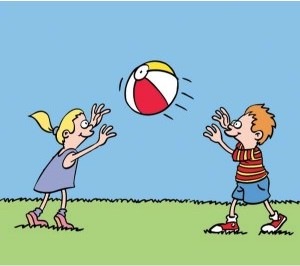
\includegraphics[width=0.25\columnwidth]{figures/I21.jpg}} \\
\hline
What is the girl doing? & What is the boy doing? & What is the boy doing? \\
\hline
\end{tabular}
%\caption{\label{tab:example-pdt-items} PDT example images with their targeted questions. In the untargeted form, the question for each is \textit{What is happening?} From left to right, the examples represent one intransitive, transitive and ditransitive item.}
\end{center}
\end{table}
\smallskip
\begin{itemize}
\pause
\item 499 participants: 358 NS (crowdsourced), 141 NNS (ESL students)
\pause
\item 30 items: Roughly 300 NS responses \& 140 NNS responses per item
\end{itemize}
\end{frame}

%\begin{frame}
%\frametitle{Task design}
%\vspace{-2ex}
%\pause
%\begin{table}
%\small
%\begin{center}
%\begin{tabular}{c r}
%& \multirow{3}{*}{
\includegraphics[width=0.22\columnwidth]{figures/rake.png}} \\
%     \multirow{3}{*}{The importance of task design; one example:} & \\
%& \\
%& \\
%What is the man doing? & \\
%\end{tabular}
%\end{center}
%\end{table}
%\pause
%NS responses:
%\begin{itemize}
%\pause
%\item He's \textbf{raking} the leaves.
%\pause
%\item The man is \textbf{raking} leaves.
%\end{itemize}
%\pause
%\smallskip
%NNS responses:
%\pause
%\begin{itemize}
%\item The man is cleaning the yard.
%\pause
%\item He is piling up leaves.
%\end{itemize}
%\smallskip
%\pause
%This is a coverage problem for my approach.
%\pause
%
%Solution? \pause Ask NS for \textbf{two} different responses.
%\end{frame}

\begin{frame}
\frametitle{Data collection}

NTS:

Explain:
\begin{itemize}
\item{targeted vs untargeted}
\item{familiar vs crowdsourced}
\item{first vs second responses}
\end{itemize}
Describe:
\begin{itemize}
\item{participants, resulting dataset: total responses, demographics}
\end{itemize}
\end{frame}

\begin{frame}
\frametitle{Annotation Features}
\pause
Feature requirements:
\begin{itemize}
\pause
\item \textit{reliablity}: consistently annotated by multiple humans;
\pause
\item \textit{validity}: directly testing for the desired constructs;
\end{itemize}
\pause
First iteration: \textbf{accuracy (A)} \& \textbf{native-likeness (NL)}
\begin{itemize}
\pause
\item \textbf{2}: $+$A, $+$NL $>$ \textbf{1}: $+$A, $-$NL $>$ \textbf{0}: $-$A, $-$NL
\pause
\item Not operationalizable: e.g., response is accurate w.r.t. prompt but adds unverifiable details; is this still \textit{accurate}?
\end{itemize}
\pause
Several iterations later; 5 binary features:
\begin{itemize}
\pause
\item \textbf{Core event}: \pause captures main action
\pause
\item \textbf{Answerhood}: \pause directly answers prompt
\pause
\item \textbf{Grammaticality}: \pause no grammar problems
\pause
\item \textbf{Interpretability}: \pause evokes clear mental image
\pause
\item \textbf{Verifiability}: \pause info is supported by image
\end{itemize}


\end{frame}

\begin{frame}
\frametitle{Annotation}
\begin{table}[htb!]
\small
\begin{center}
%\begin{tabular}{|p{3.7cm}|c|c|c|c|c|}
\begin{tabular}{|l|c|c|c|c|c|}
\hline
\multicolumn{6}{|c|}{
\includegraphics[width=0.25\columnwidth]{figures/I02.jpg}} \\
\hline
\textit{What is the boy doing?} & C & A & G & I & V \\
\hline
\hline
He is eating food. & 0 & 1 & 1 & 1 & 1 \\
\hline
he eating pizza. & 1 & 1 & 0 & 1 & 1 \\
\hline
The boy is smiling pizza. & 0 & 1 & 0 & 0 & 0 \\
\hline
He may get fat eating. & 0 & 0 & 1 & 1 & 0 \\
\hline
\end{tabular}
\caption{\label{tab:dev-transitive} \small Annotated for five features: Core event (\textit{C}), Answerhood (\textit{A}), Grammaticality (\textit{G}), Interpretability (\textit{I}) and Verifiability (\textit{V}).}
\end{center}
\end{table}
\end{frame}

\begin{frame}
\frametitle{Feature reliability}
\pause
Inter-rater reliability for two annotators and 10\% of the dataset:
\pause

\textit{yes} annotations for Annotator 1 (note skewedness), expected chance agreement (\textit{Chance}), actual observed agreement (\textit{Observed}) and Cohen's kappa (\textit{Kappa})

\begin{table}[htb!]
\begin{center}
\begin{tabular}{|l|l||l|l||l|}
\hline
Set	& A1Yes & Chance & Observed & Kappa \\
\hline
\hline
Core Event & 0.733 & 0.601 & 0.923 & 0.808 \\
\hline
Answerhood & 0.834 & 0.721 & 0.982 & 0.936 \\
\hline
Grammaticality & 0.861 & 0.768 & 0.960 & 0.827 \\
\hline
Interpretability & 0.818 & 0.682 & 0.919 & 0.744 \\
\hline
Verifiability & 0.845 & 0.719 & 0.968 & 0.884 \\
\hline
\pause \\
\hline
Intransitive & 0.863 & 0.758 & 0.978 & 0.910 \\
\hline
Transitive & 0.780 & 0.653 & 0.949 & 0.853 \\
\hline
Ditransitive & 0.812 & 0.678 & 0.924 & 0.764 \\ 
\hline
\end{tabular}
\end{center}
\end{table}
\end{frame}

\begin{frame}
\frametitle{Weighting features}
\pause
\begin{itemize}
\item Features do not contribute equally to response ``goodness''
\pause
\item Raters perform holistic preference test (with annotations hidden)
\end{itemize}
\pause
\vspace{-2ex}
\begin{table}
\scriptsize
\begin{center}
\begin{tabular}{|=l|+c||+c|+c|+c|+c|+c|}
\hline
\textit{What is the boy doing?} & Pref? & C & A & G & I & V \\
\hline
\hline
\rowstyle{\color{RoyalBlue}}He is eating food. & \textbf{yes} & \textbf{0} & \textbf{1} & \textbf{1} & \textbf{1} & \textbf{1} \\
\hline
\rowstyle{\color{Maroon}}He may get fat eating. & no & 0 & 0 & 1 & 1 & 0 \\
\hline
\pause \\
\hline
\only<2->{\rowstyle{\color{Maroon}}He is hungry. & no & 0 & 0 & 1 & 0 & 1} \\
\hline
\uncover<2->{\rowstyle{\color{RoyalBlue}}the boy is eating pizza & \textbf{yes} & \textbf{1} & \textbf{1} & \textbf{1} & \textbf{1} & \textbf{1}} \\
\hline
\pause \\
\hline
\only<3->{\rowstyle{\color{RoyalBlue}}The child is about to eat pizza. & \textbf{yes} & \textbf{1} & \textbf{0} & \textbf{1} & \textbf{1} & \textbf{1}} \\
\hline
\uncover<3->{\rowstyle{\color{Maroon}}he eating. & no & 0 & 1 & 0 & 1 & 1} \\
\hline
\pause \\
\hline
\only<4->{\rowstyle{\color{RoyalBlue}}Totals preferred responses & & 2 & 2 & 3 & 3 & 3} \\
\hline
\uncover<4->{\rowstyle{\color{Maroon}}Totals dispreferred responses & & 0 & 1 & 2 & 2 & 2 \\
\hline
\rowstyle{\color{RoyalBlue}}Net preferred (pref {\color{black}-} {\color{Maroon}dispref}) & & 2 & 1 & 1 & 1 & 1 \\
\hline
Feature weight &  & .333 & .167 & .167 & .167 & .167} \\
\hline \pause \\
%\multicolumn{7}{c}{} \\
\hline
\only<5->{}
\uncover<5->{$^*$Real feature weight &  & .365 & .093 & .055 & .224 & .263} \\
\hline
\end{tabular}
\end{center}
\end{table}
\end{frame}

\begin{frame}
\frametitle{Preference reliability (feature weights)}
\begin{table}[htb!]
\begin{center}
\begin{tabular}{|l|l|l|}
\hline
 Chance Agree & Observed Agree & Kappa \\
\hline
0.621 & 0.883 (265/300) & 0.692 \\
\hline
\end{tabular}
\caption{\label{tab:ABAgreement} Preference task agreement scores for two annotators on a sample of 300 response pairs; expected chance agreement, observed agreement and Cohen's Kappa.}
\end{center}
\end{table}

\end{frame}

\begin{frame}
\frametitle{Weighted annotation scores}
\small
\begin{itemize}
\pause
\item Calculate weighted annotation score (S_{wa}) for each NNS response;
\pause
\item Rank by S_{wa} ($\rightarrow$ R_{wa}); use this as gold standard or benchmark;
\pause
\begin{itemize}
\item Score system output: R_{wa} vs. system ranking $\rightarrow$ Spearman $\rho$
\end{itemize}
\end{itemize}
\pause
\begingroup
\setlength{\tabcolsep}{4pt} % Default value: 6pt
\begin{table}
%\tiny
%\begin{table}[t!] This line is giving me trouble when I go to typeset
\begin{center}
%\begin{tabular}{|p{3.7cm}|c|c|c|c|c|}
\begin{tabular}{|l|c|c|c|c|c||l|c|}
%\hline
%\multicolumn{6}{|c|}{
\includegraphics[width=0.45\columnwidth]{figures/I02.jpg}} \\
%\multicolumn{6}{|c|}{
\includegraphics[width=0.3\columnwidth]{figures/I02.jpg}} \\
\hline
%\multicolumn{3}{|l|}{What is the woman doing? [Intransitive]} \\
\textit{What is the boy doing?} & C & A & G & I & V & S_{wa} & R_{wa} \\
\hline
\hline
The boy is eating. & 0 & 1 & 1 & 1 & 1 & 0.635 & 4 \\
\hline
A baby is eating pizza & 0 & 0 & 1 & 1 & 0 & 0.279 & 5 \\
\hline
The boy enjoys his pizza. & 1 & 0 & 1 & 1 & 1 & 0.907 & 2 \\
\hline
the boy is eating pizza & 1 & 1 & 1 & 1 & 1 & 1.0 & 1 \\
\hline
The kid is eats pizza & 1 & 0 & 0 & 1 & 1 & 0.852 & 3 \\
\hline
\end{tabular}
%\caption{\label{tab:dev-transitive} \scriptsize Annotated for five features: Core event (\textit{C}), Verifiability (\textit{V}), Answerhood (\textit{A}), Interpretability (\textit{I}) and Grammaticality (\textit{G}).}
\end{center}
\end{table}
\endgroup

\end{frame}

\begin{frame}
\frametitle{Analyzing NNS responses}
\small
At this point, my goal is a system that scores and ranks NNS responses via comparison with the crowdsourced NS responses. The system produced ranking should correlate highly with the R_{wa}.

\bigskip

If particular system configuration settings correlate highly with item features (intransitive / transitive / ditransitive; response complexity), I can optimize the system for new items.
\end{frame}

\begin{frame}
\frametitle{Analyzing NNS responses}
\small
The system works like this; for each item:

\medskip
Generate a NS model:
\begin{enumerate}
\item dependency parse the collection of NS responses;
\item get tf-idf score for each unique dependency (via a large balanced corpus).
\end{enumerate}

\medskip

Score each NNS response:
\begin{enumerate}
\item As above: dependency parse, tf-idf;
\item Compare NS vs NNS tf-idf vectors: 1 - cosine $=$ response score.
\end{enumerate}

Finally, the NNS responses are ranked by score, and the Spearman rank correlation between R_{wa} and the system is taken as the system configuration score for the item.

\bigskip

By selecting different parameter settings in this approach, I arrive at 12 different system configurations. Each configuration scores and ranks all NNS responses.

\end{frame}

\begin{frame}
\frametitle{System configurations}
\small

Consider this simplified set of 2 parameters $x$ 2 settings $=$ 4 configurations.
\medskip

\begin{itemize}
\item \textbf{Dependency format}:
\begin{itemize}
\item \textbf{labeled}: e.g., nsubj(eat,boy); nobj(eat,pizza)
\item \textbf{unlabeled}: e.g., $\langle$null$\rangle$(eat,boy); $\langle$null$\rangle$(eat,pizza)
\end{itemize}
\smallskip

\item \textbf{NS response model}:
Note: Each NS participant gave \textit{two} responses per PDT item
\begin{itemize}
\item \textbf{first}: Model contains only the first response from NS
\item \textbf{mixed}: Model is half first reponses and half second responses
\end{itemize}
\end{itemize}
\begin{table}[htb!]
\small
\begin{center}
%\begin{tabular}{|p{3.7cm}|c|c|c|c|c|}
\begin{tabular}{|l||l|l|}
\hline
dep\textbackslash model & first & mixed \\
\hline
\hline
labeled & lab\_first & lab\_mixed \\
\hline
unlabeled & unlab\_first & unlab\_mixed \\
\hline
\end{tabular}
%\caption{\scriptsize Four system configurations for scoring NNS responses.}
\end{center}
\end{table}

\end{frame}


\begin{frame}
\frametitle{System configurations}
\small
\begin{itemize}
\item Score \& rank NNS responses using different configurations;
\item Compare with R_{wa} to get a Spearman correlation.
\end{itemize}
\begingroup
\setlength{\tabcolsep}{4pt} % Default value: 6pt
\begin{table}
\begin{center}
\begin{tabular}{|l||l|c||l|c||l|c|}
\hline
NNS & S_{wa} & R_{wa} & S_{lf} & R_{lf} & S_{uf} & R_{uf} \\
\hline
\hline
p1 & 0.63 & 4 & 0.53 & 4 & 0.11 & 5 \\
\hline
p2 & 0.27 & 5 & 0.13 & 5 & 0.15 & 4 \\
\hline
p3 & 0.90 & 2 & 0.91 & 1 & 0.68 & 1 \\
\hline
p4 & 1.0 & 1 & 0.80 & 2 & 0.41 & 2 \\
\hline
p5 & 0.85 & 3 & 0.77 & 3 & 0.20 & 3 \\
\hline
\hline
\multicolumn{3}{|l||}{Spearman $\rho$} & \multicolumn{2}{r||}{.899} & \multicolumn{2}{r|}{.799} \\
\hline
\multicolumn{3}{|l||}{Spearman p-val} & \multicolumn{2}{r||}{.037} & \multicolumn{2}{r|}{.104}  \\
\hline
\end{tabular}
%\caption{\label{tab:modelranks} Response scores and ranks for: weighted annotation; system configurations: labeled\_first (\textit{lf}) and unlabeled\_first (\textit{uf}).}
\end{center}
\end{table}
\begin{itemize}
\item \textit{lf} is \textit{labeled\_first}; \textit{uf} is \textit{unlabeled\_first}:
\item \textit{labeled} for labeled dependencies (vs. \textit{unlabeled})
\item \textit{first} for models containing only the first response from NS (vs a \textit{mix} of first and second responses)
\end{itemize}
\endgroup
\end{frame}

\begin{frame}
\frametitle{Results \& Optimization}
NTS: Multiple slides; describe most salient findings
\end{frame}

\begin{frame}
\frametitle{Summary}
NTS: one slide
\end{frame}

\begin{frame}
\frametitle{Outlook}
NTS: one slide
\end{frame}

%\begingroup
%\setlength{\tabcolsep}{4pt} % Default value: 6pt
%\begin{table}
%\begin{center}
%\begin{tabular}{|l||l|c||l|c||l|c||l|c||l|c|}
%\hline
%P & S_{wa} & R_{wa} & S_{lf} & R_{lf} & S_{uf} & R_{uf} & S_{lm} & R_{lm} & S_{um} & R_{um} \\
%\hline
%\hline
%p1 & 0.63 & 4 & 0.53 & 4 & 0.11 & 5 & 0.29 & 4 & 0.39 & 3 \\
%\hline
%p2 & 0.27 & 5 & 0.13 & 5 & 0.15 & 4 & 0.15 & 5 & 0.53 & 5 \\
%\hline
%p3 & 0.90 & 2 & 0.91 & 1 & 0.68 & 1 & 0.33 & 3 & 0.55 & 1 \\
%\hline
%p4 & 1.0 & 1 & 0.80 & 2 & 0.41 & 2 & 0.70 & 1 & 0.24 & 2 \\
%\hline
%p5 & 0.85 & 3 & 0.77 & 3 & 0.20 & 3 & 0.63 & 2 & 0.22 & 4 \\
%\hline
%\end{tabular}
%\caption{\label{tab:modelranks} Response scores and ranks for: weighted annotation; system configurations: labeled\_first (\textit{lf}), unlabeled\_first (\textit{uf}), labeled\_mixed (\textit{lm}), unlabeled\_mixed (\textit{um}).}
%\end{center}
%\end{table}
%\endgroup
%\end{frame}

%\begin{frame}
%\frametitle{Finding trends}
%From the full set of 360 Spearman correlation scores, I used various subsets of scores to generate hierarchical clusters of the 30 items. I've found some clustering according to verb type (intransitive, transitive or ditransitive), but this trend is not very strong.
%
%\medskip
%
%\medskip
%I'm currently exploring features other than verb type to see if they correlate with Spearman and can thus help predict optimal system configurations for new items. These features relate to item complexity: type-to-token ratios for the collection of NS responses; mean/median leave-one-out system scores for the NS collection.
%\end{frame}
%
%\begin{frame}
%\frametitle{Future directions}
%Other predictive features: image complexity (compression; entropy)
%
%\medskip
%
%Feedback: Responses scoring below a threshold should be ``recast'' as the most similar NS response (with S_{wa} $=$ 1).
%
%Augment this with SBERT but rely on my system to find appropriate feedback.
%
%\medskip
%
%For some contexts (e.g., tutoring vs testing), an oracle ranking by the \textit{core event} feature alone may be preferable. Because the feature is binary, Spearman would not be appropriate, so average precision or T-test scores could be used to optimize configurations.
%
%\medskip
%
%My NNS participants were $>$90\% L1 Chinese. I'd love to have an equivalent dataset for another L1 for comparison and to attempt L1-specific optimization.
%
%\end{frame}
%
%\begin{frame}
%\frametitle{Generalizing}
%
%In a globalized world, we need to be able to analyze speech and text from NNS of English (and other languages). In high stakes contexts, processing should be adaptable, able to abstract from surface form to meaning, and maintain a degree of transparency and explainability. 
%
%\end{frame}



\begin{beamercolorbox}{title}
\mbox{}\\[1ex]%\vspace{1ex}
\usebeamerfont{title}References
\end{beamercolorbox}
\medskip
\scriptsize
\bibliographystyle{styles/myaclnat}
\bibliography{levi-bib}

\end{document}